%========================================================================================
% Compilation should work with PDFLaTeX
%========================================================================================
% Type of document and general formatting
\documentclass[a4paper,11pt]{article}

\usepackage[left=2.5cm,right=2.5cm,top=2.5cm,bottom=2.5cm]{geometry}
\linespread{1.25}

%========================================================================================
% These packages are for language and font settings
\usepackage[english,activeacute]{babel} % Language
\usepackage{tgpagella}					% Text font
\usepackage[T1]{fontenc}				% T1 Encoding of font
\usepackage[utf8]{inputenc}				% Special symbols
\usepackage{lmodern}


%========================================================================================
\usepackage[sc]{mathpazo}				% Math font
\usepackage{amsmath,amsfonts,amssymb}	% Math symbols
\usepackage{dsfont}						% Math symbols like R for reals...
\usepackage{amsthm}						% For theorem styles
\usepackage{siunitx}

%========================================================================================
% Other packages
\usepackage{graphicx}
\usepackage{longtable}
\usepackage[svgnames]{xcolor}

%========================================================================================
\usepackage{accents}
\newcommand*{\dt}[1]{%
	\accentset{\mbox{\large\bfseries .}}{#1}} % Larger dot for time derivative


\usepackage{hyperref}
\hypersetup
{
    pdfauthor={Rafael Serrano-Quintero},
    pdfsubject={Structural Transformation in Indian Services},
    colorlinks = {true},
    linkcolor = {FireBrick},
    citecolor = {FireBrick},
    urlcolor = {RoyalBlue},
}

\usepackage{appendix}
\usepackage{marvosym}
\usepackage{enumerate} %For enumerating with letters with option [a)]
\usepackage{fancyvrb}  %To reduce font size in verbatim environment
\usepackage{epstopdf}
\usepackage[flushleft]{threeparttable}
\usepackage{pdflscape}
\usepackage{natbib}
\usepackage{subcaption}
\usepackage{booktabs}
\usepackage[super]{nth}
\usepackage{float}

\newcommand{\source}[1]{\caption*{\tiny Source: {#1}} }

%========================================================================================
% Stata Preamble for Tables
%========================================================================================

\newcommand{\sym}[1]{\rlap{#1}}% Thanks to David Carlisle

\let\estinput=\input% define a new input command so that we can still flatten the document

\newcommand{\estwide}[3]{
		\vspace{.75ex}{
			\begin{tabular*}
			{\textwidth}{@{\hskip\tabcolsep\extracolsep\fill}l*{#2}{#3}}
			\toprule
			\estinput{#1}
			\bottomrule
			\addlinespace[.75ex]
			\end{tabular*}
			}
		}	

\newcommand{\estauto}[3]{
		\vspace{.75ex}{
			\begin{tabular}{l*{#2}{#3}}
			\toprule
			\estinput{#1}
			\bottomrule
			\addlinespace[.75ex]
			\end{tabular}
			}
		}

% Allow line breaks with \\ in specialcells
	\newcommand{\specialcell}[2][c]{%
	\begin{tabular}[#1]{@{}c@{}}#2\end{tabular}}

% *****************************************************************
% Custom subcaptions
% *****************************************************************
% Note/Source/Text after Tables
\newcommand{\figtext}[1]{
	\vspace{-1.9ex}
	\captionsetup{justification=justified,font=footnotesize}
	\caption*{\hspace{6pt}\hangindent=1.5em #1}
	}
\newcommand{\fignote}[1]{\figtext{\emph{Note:~}~#1}}

\newcommand{\figsource}[1]{\figtext{\emph{Source:~}~#1}}

% Add significance note with \starnote
\newcommand{\starnote}{\figtext{* p < 0.1, ** p < 0.05, *** p < 0.01. Standard errors in parentheses.}}

% *****************************************************************
% siunitx
% *****************************************************************
\usepackage{siunitx} % centering in tables
	\sisetup{
		detect-mode,
		tight-spacing           = true,
		group-digits            = false ,
		input-signs             = ,
		input-symbols           = ( ) [ ] - + *,
		input-open-uncertainty  = ,
		input-close-uncertainty = ,
		table-align-text-post   = false
        }

% Document parameters
\title{Chapter 1: Single Variable Functions}
\author{Rafael Serrano Quintero \\
Dpt. Fundamentos del An\'alisis Econ\'omico \\
University of Alicante}
\date{}        

\theoremstyle{definition}
\newtheorem{definition}{Definition}
\newtheorem{example}{Example}
\theoremstyle{plain}
\newtheorem{theorem}{Theorem}
\newtheorem{lemma}{Lemma}
%========================================================================================
					% === Title, thanks, and author data === %
%========================================================================================

\begin{document}      

\maketitle

    
\section{Single Variable Functions:
Continuity}\label{single-variable-functions-continuity}


\subsection{Basic concepts: Domain, Range, and Graph of a
Function}\label{basic-concepts-domain-range-and-graph-of-a-function}

\subsubsection{Previous concepts}\label{previous-concepts}

Real line: types of numbers 

\begin{itemize}
	\item Natural numbers \((\mathbb{N})\): \(0,1,2,3,4,5,\ldots\) 
	\item Integers \((\mathbb{Z})\): \(\ldots,-5,-4,-3,-2,-1,0,1,2,3,4,5,\ldots\) 
	\item Rational numbers \((\mathbb{Q})\): \(\frac{a}{b},a,b\in\mathbb{Z},b\neq 0\) 
	\item Irrational numbers \((\mathbb{I}\)): \(\sqrt{2}\approx 1.41, \pi\approx 3.14,e \approx 2.72\ldots\) 
	\item Real numbers \((\mathbb{R})\): \(\mathbb{Q}\cup\mathbb{I}\)
\end{itemize}

Intervals of real numbers:

\begin{itemize}
\item
  Open interval: \((a,b) := \{x\in\mathbb{R}:a<x<b\}\)
\item
  Closed interval: \([a,b] := \{x\in\mathbb{R}:a\leq x\leq b\}\)
\item
  Half open interval: \((a,b] := \{x\in\mathbb{R} : a<x\leq b\}\)
\item
  Unbounded interval:
  \((a,+\infty) := \{x\in\mathbb{R} : a < x < +\infty\}\)
\end{itemize}

\begin{theorem} 
No number \(r\in\mathbb{Q}\) has square equal to
\(2\); i.e. \(\nexists r\in\mathbb{Q} : r^2 = 2\), i.e., \(\sqrt{2}\notin\mathbb{Q}\).
\end{theorem}

\begin{proof}
To prove that every \(r\) has \(r^2\neq 2\) we can use
the actual definition of rational numbers, that is, we know we can
express \(r = \frac{p}{q}\) where \(p,q\in\mathbb{Z}\) and \(q\neq 0\).
Thus, to prove the theorem we could show that \(p^2\neq 2q^2\).


\begin{itemize}
\item
  Assumption: \(p\) and \(q\) have no common factors, since we could've
  canceled out beforehand.
\end{itemize}

\emph{Case 1:} \(p\) is odd. Then, \(p^2\) is also odd, but \(2q^2\) is
\textbf{not} odd. Then, \(p^2\neq 2q^2\).

\emph{Case 2:} \(p\) is even. Since \(p\) and \(q\) have \textbf{no
common factors}, \(q\) is odd. Then \(p^2\) is divisible by \(4\) while
\(2q^2\) is not. Therefore, \(p^2\neq 2q^2\).

Since
\(p^2\neq 2q^2 \forall p\in\mathbb{Z}\Rightarrow \nexists r = p / q \ : \ r^2 = 2\)
\end{proof}

\begin{definition}
Absolute value of a number: three equivalent definitions

\begin{enumerate}
\def\labelenumi{\arabic{enumi}.}
\item
  \[
  \lvert x \rvert =
  \begin{cases}
  \phantom{-}x & \text{if} \ x\geq 0 \\
  -x & \text{if} \ x < 0 
  \end{cases}
  \]
\item
  \[
  \lvert x \rvert = + \sqrt{x^2}
  \]
\item
  \[
  \lvert x \rvert = \text{max}\{x, -x\}
  \]
\end{enumerate}
\end{definition}


Using the absolute value, we can define subsets of real numbers:

\begin{itemize}
	\item
  Open interval with \textbf{center} \(a\) and \textbf{radius} \(r\):
  \(\{x\in\mathbb{R} : \lvert x-a \rvert < r\} = (a-r,a+r)\)
\item
  Closed interval with \textbf{center} \(a\) and \textbf{radius} \(r\):
  \(\{x\in\mathbb{R} : \lvert x-a \rvert \leq r\} = [a-r,a+r]\)
\item
  Complementaries: \[
  \{x\in\mathbb{R} : \lvert x-a \rvert > r\} = \mathbb{R}\setminus\{x\in\mathbb{R}: \lvert x-a \rvert \leq r\} = (-\infty,a-r)\cup(a+r,+\infty)
  \]
\end{itemize}

\[
\{x\in\mathbb{R} : \lvert x-a \rvert \geq r\} = \mathbb{R}\setminus\{x\in\mathbb{R}: \lvert x-a \rvert < r\} = (-\infty,a-r]\cup[a+r,+\infty)
\]

\begin{example}
Determine the following sets expressing them in
interval or union of intervals form:
\end{example}

\begin{enumerate}
\def\labelenumi{\arabic{enumi}.}
\item
  \(\{x\in\mathbb{R} : \lvert x-3\rvert > 2\}\); \textbf{Solution:}
  \((-\infty,1)\cup(5,+\infty)\)
\item
  \(\{x\in\mathbb{R} : \lvert x+1\rvert \geq 5\}\); \textbf{Solution:}
  \((-\infty,-6]\cup[4,+\infty)\)
\item
  \(\{x\in\mathbb{R} : \lvert x-2\rvert \leq 8\}\); \textbf{Solution:}
  \([-6,10]\)
\end{enumerate}

\begin{theorem}{\textbf{Triangle Inequality:}}
For all \(x,y\in\mathbb{R}\) we have
\(\lvert x+y \rvert \leq \lvert x \rvert + \lvert y \rvert\).
\end{theorem} 


\begin{proof}
By transitivity (\(x<y<z\Rightarrow x<z\)) and
translation (\(x<y\Rightarrow x+z < y+z\)) properties, we have that:

\[
x+y \leq \lvert x \rvert + y \leq \lvert x \rvert + \lvert y \rvert
\]

\[
-x-y \leq \lvert x \rvert - y \leq \lvert x \rvert + \lvert y \rvert
\]

Since

\[
\lvert x + y\rvert \begin{cases} 
x + y & \text{if } x+y \geq 0 \\
-x-y  & \text{if } x+y \leq 0
\end{cases}
\]

And both \(x+y\) and \(-x-y\) are less than or equal to
\(\lvert x \rvert + \lvert y \rvert\), we infer that
\(\lvert x + y \rvert \leq \lvert x \rvert + \lvert y \rvert\).
\end{proof}


\begin{definition}
The \textbf{neighborhood} of a point \(a\) is an
(open) interval with center \(a\) and a radius \(\varepsilon\) (small
close to \(0\)).

\[
\mathcal{E}(a,\varepsilon) \{x\in\mathbb{R} : \lvert x-a\rvert < \varepsilon\} = (a-\varepsilon,a+\varepsilon)
\]
\end{definition}

\subsubsection{Cartesian Coordinates: Origin, Axes, Points in the
Plane}\label{cartesian-coordinates-origin-axes-points-in-the-plane}

\begin{itemize}
	\item
  Plane \(\mathbb{R}\) is the set of ordered pairs of real numbers
  \((x,y)\) where \(x,y\in\mathbb{R}\)
\item
  Horizontal axis (abscissa) is formed by the points:
  \(X = \{(x,0) : x\in\mathbb{R}\}\)
\item
  Vertical axis (ordinate) is formed by the points:
  \(Y = \{(0,y) : y\in\mathbb{R}\}\)
\end{itemize}

\subsubsection{Lines in the plane}\label{lines-in-the-plane}

\begin{definition}
A \textbf{line} is every set in the plane of the
form \(\{(x,y)\in\mathbb{R}^2 : Ax + By = c\}\) where \(A,B,c\) are
known real numbers, with \(A,B \neq 0\).
\end{definition}

\begin{example}
Represent the following lines in the plane:

\begin{enumerate}
\def\labelenumi{\arabic{enumi}.}
\item
  \(x+y=1\)
\item
  \(y=2x\)
\item
  \(x=8\)
\item
  \(y=-2\)
\end{enumerate}
\end{example}

\begin{figure}[htbp]
	\centering 
		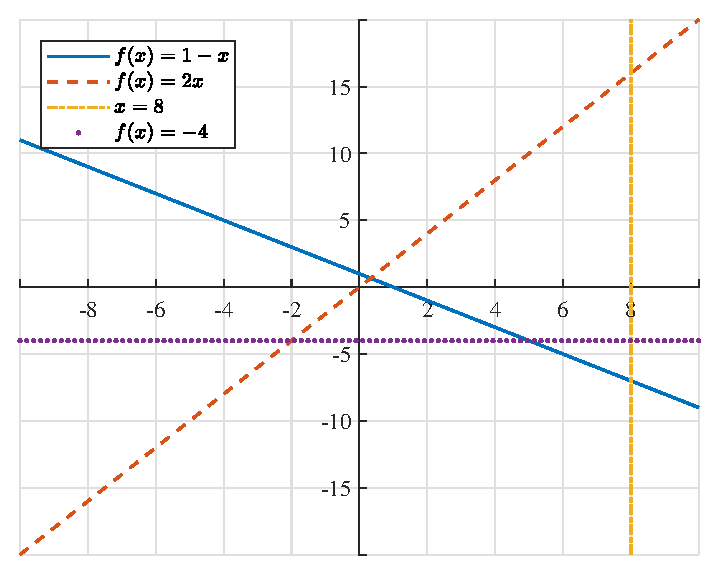
\includegraphics[width = 0.65\textwidth]{Ch1_files/Ch1_2_0.eps} 
		\caption{Representing Lines}
		\label{fig:representing_lines}
\end{figure}    

\subsubsection{Slope of a line: Meaning}\label{slope-of-a-line-meaning}

The main characteristic which distinguishes one line from another is its
steepness, the steepness is also called \textbf{slope}. If a line is
upward sloped, graphically, the line goes up (the function is
\textbf{increasing}), if the line is downward sloped, it goes down (the
function is \textbf{decreasing}).

\begin{definition} 
Let the line be \(f(x) = a + m x\) where
\(a,b\in\mathbb{R}\). Let \((x_0,y_0),(x_1,y_1)\) be two arbitrary
points on a line \(\ell\). The \emph{ratio}

\[
m = \frac{y_1-y_0}{x_1-x_0} = \frac{\Delta f(x)}{\Delta x}
\]

is called the \textbf{slope} of line \(\ell\). Then, the slope \(m\) is
defined as the \emph{ratio} of the amount of units that \(f(x)\)
increases by the amount of units that \(x\) increases. For lines, the
slope is independent of the two points chosen on \(\ell\).
\end{definition}

    \begin{figure}[htbp]
    	\centering 
    		\includegraphics[width = 0.65\textwidth]{Ch1_files/Ch1_4_0.png}
    		\caption{Differences in Slope}
    		\label{fig:slopes_origin}
    \end{figure}
    

\textbf{Independence of the Points}

The slope of a linear function is independent of the points chosen

    \begin{figure}[htbp]
    	\centering 
    		\includegraphics[width = 0.65\textwidth]{Ch1_files/Ch1_6_0.png}
    		\caption{Slope Independence for Linear Functions}
    		\label{fig:independence_slope}
    \end{figure}

\subsubsection{Equation of a Line}\label{equation-of-a-line}

\begin{enumerate}
\def\labelenumi{\arabic{enumi}.}
\item
  Given a point \((x_1, y_1)\) and the slope \(m\), the equation of a
  line is given by: \[
  y - y_1 = m(x - x_1)
  \] 
  \[
  y = \underset{a}{\underbrace{(y_1 - m x_1)}} + m x = a + mx
  \]
\item

 Given two points \((x_1,y_1),(x_2, y_2)\)

  \begin{enumerate}
  \def\labelenumii{\arabic{enumii}.}
 
   \item
    First we compute the slope as
    \(m = \frac{\Delta y}{\Delta x} = \frac{y_2 - y_1}{x_2 - x_1}\)
  \item
    We choose any of the two known points and apply previous formula.
  \item
    If the line turns to be vertical, the denominator will be \(0\) but,
    in this case, we have \(x_2 = x_1\) and the equation for a vertical
    line is just \(x = x_1\).
  \end{enumerate}
\end{enumerate}

\begin{example} 
Compute the equation of the following lines and draw
them.

\begin{enumerate}
\def\labelenumi{\arabic{enumi}.}
\item
  The line that goes through point \((2, -1)\) with slope \(m = 5\) \[
  y - (-1) = 5(x - 2) \Rightarrow y = 5x - 11
  \]
\item
  The line that goes through points \((2, -1)\) and \((-1,2)\) \[
  m = \frac{\Delta y}{\Delta x} = \frac{2-(-1)}{-1-2} = \frac{3}{-3} = -1 
  \] Applying
  \(y - y_1 = m(x - x_1) \Rightarrow y-(-1) = (-1)(x-2) \Rightarrow y = -x + 1\)
\end{enumerate}
\end{example}

\subsubsection{Euclidean Vector}\label{euclidean-vector}

A Euclidean (geometric or spatial) vector is a geometric object that has
\textbf{magnitude} and \textbf{direction}.

Two points in a plane define a unique line. If we subtract coordinate by
coordinate:

\[
\vec{\mathbf{u}} = (x_1, y_1) - (x_2, y_2) = (x_1 - x_2, y_1 - y_2)
\]

This latter vector indicates the \emph{direction} the line follows.
Thus, the equation of a line can be \emph{parametrically} written as:

\[
\{(x,y)\in\mathbb{R}^2 : (x, y) = (x_1, y_1) + \lambda\vec{\mathbf{u}}, \ \lambda\in\mathbb{R}\}
\]

\begin{example} 
Euclidean vector and parametric equation of the line
that goes through the points \((2,5)\) and \((0,3)\).

\begin{enumerate}
\def\labelenumi{\arabic{enumi}.}
\item
  The Euclidean vector is given by
  \(\vec{\mathbf{u}} = (2,5)-(0,3) = (2,2)\)
\item
  The parametric equation is given by \((x,y) = (2,5) + \lambda(2,2)\)
\end{enumerate}

To obtain the standard Cartesian equation of the line from the
parametric equation, we just need to solve for \(\lambda\) in one of the
coordinates and substitute in the other. For this example, the Cartesian
equation is given by \(y = x + 3\)
\end{example}

    \begin{figure}[htbp]
    	\centering 
    		\includegraphics[width = 0.65\textwidth]{Ch1_files/Ch1_8_0.png}
    		\caption{Representation of the Line and its Euclidean Vector}
    		\label{fig:euclidean_vector}
    \end{figure}
    
Note that if we have a line given by \(y = a + m x\), we know it will go
through the points \((0,a)\) and \((1, m+n)\) so we can easily obtain
both the Euclidean vector \(\vec{\mathbf{u}}\) and the parametric form
of this equation.

\subsubsection{A Snippet of
Trigonometry}\label{a-snippet-of-trigonometry}

Given an angle \(\alpha\), the main trigonometric functions are given
by:

\[\sin(\alpha) = \frac{BA}{BO} \ \cos(\alpha) = \frac{AO}{BO} \ \tan(\alpha) = \frac{\sin(\alpha)}{\cos(\alpha)} = \frac{BA}{AO}\]

Where $BA,BO,AO,BA$ are the distances represented in Figure \ref{fig:trig_relationships}.

    \begin{figure}[htbp]
    	\centering 
    		\includegraphics[width = 0.65\textwidth]{Ch1_files/Ch1_10_0.png}
    		\caption{Trigonometric Relationships}
    		\label{fig:trig_relationships}
    \end{figure}
    
    Angles are measured in \emph{radians}. A circle has \ang{380} which
corresponds to \(2\pi\) radians.

As a direct consequence of \textbf{Pythagorean Theorem} we get the
\emph{fundamental relationship} between sinus and cosinus. Exercise \ref{exercise-3} asks you to prove it.

\[
\sin^2(\alpha) + cos^2(\alpha) = 1
\]

Let's plot the \(\sin\) and \(\cos\) functions in Figure \ref{fig:sin_cos}.

    \begin{figure}[htbp]
    	\centering 
    		\includegraphics[width = 0.65\textwidth]{Ch1_files/Ch1_12_0.png}
    		\caption{$\sin$ and $\cos$ functions}
    		\label{fig:sin_cos}
    \end{figure}
    
    \subsubsection{Functions of a Real
Variable}\label{functions-of-a-real-variable}

\begin{definition} 
A \textbf{function} \(f\) is a rule that assigns to
each number \(x\) in a set \(\mathcal{D}\subseteq\mathbb{R}\) a number
in \(\mathbb{R}\) denoted by \(f(x)\). The number \(y = f(x)\) is called
the \textbf{image} of \(x\) under \(f\). The pair formed by each real
number \(x\) and its image \(f(x)\) determines a point \((x, f(x))\) in
the plane \(\mathbb{R}\). The set of all these pairs is called the
\textbf{graph of a function}.

\[
G_f = \{(x,f(x))\in\mathbb{R}^2 \ ; \ x\in \mathcal{D}\}
\]

Where \(\mathcal{D}\) is the set where the function is defined, also
called \textbf{domain}.
\end{definition}

\begin{example} 
A basic example can be the \textbf{non-vertical} lines.
In this case, the equation of the line can be written as
\(y = f(x) = a + m x\). The domain of this function is
\(\mathcal{D} = \mathbb{R}\)
\end{example}

\begin{example} 
The domain of the function \(f(x) = \frac{1}{x}\) is no
longer \(\mathbb{R}\) since it is not defined for \(x = 0\). Therefore,
the domain, will be
\(\mathcal{D} = \{x\in\mathbb{R} \ : \ x\neq 0\} = \mathbb{R} - \{0\}\).
And its graph is
\end{example}

    \begin{figure}[htbp]
    	\centering 
    		\includegraphics[width = 0.65\textwidth]{Ch1_files/Ch1_14_0.png}
    \end{figure}
    
Functions can also have restricted domain depending on the application
in which the function arises.

\textbf{Example:} Suppose we have a firm with a cost function that is
linear, such as \(C(q) = a + b q\) where \(q\) is the quantity produced.
Which is the domain of this function?

The domain of the function will be
\(\mathcal{D} = \{q\in\mathbb{R}_+\} = \{q\in\mathbb{R} \ : \ q\geq 0 \}\)

\textbf{Example:} Compute the domain of the following function:

\[
f(x) = \log\left(\frac{x+2}{x-1}\right)
\]

\begin{itemize}
	\item
  The denominator \((x-1)\) needs to be different from \(0\), thus,
  \(x\neq 1\).
\item
  Logs can only be computed for positive numbers, thus, both numerator
  and denominator must have equal signs.

  \begin{itemize}
 
   \item
    Both positive \(\rightarrow x+2 > 0 \ ; x-1 > 0 \Rightarrow x > 1\)
  \item
    Both negative \(\rightarrow x+2 < 0 \ ; x-1 < 0 \Rightarrow x < -2\)
    Thus, the domain of the function is given by \[
    \mathcal{D} = (-\infty, -2)\cup(1,+\infty)
    \]
  \end{itemize}
\end{itemize}

Note that neither \(-2\) nor \(1\) can enter in the domain.

Following figure shows some points of the domain.

    \begin{figure}[htbp]
    	\centering 
    		\includegraphics[width = 0.65\textwidth]{Ch1_files/Ch1_16_0.png}
    \end{figure}
    

\subsection{Inverse Function}\label{inverse-function}

\subsubsection{Composite functions}\label{composite-functions}

\begin{definition} 
Given two functions $f,g \ : \ \mathbb{R} \rightarrow \mathbb{R}$, the \textbf{composite} function of $f$ with $g$ denoted by $(f\circ g)(x)$ is a new function
defined by:

\[
(f\circ g)(x) = f(g(x))
\]

That is, a new number obtained by first applying $g$ to $x$ and $f$ to the result of that.
\end{definition}

\begin{example} 
Take the profit function of a firm \(\Pi\) which is
generally a function of the output. Suppose that the profit of a firm is
given by

\[
\Pi(y) = y^2 - y + 2
\]

And the production function of the firm is $y = f(k) = k^{\alpha}$. Where $y$ is output, and $k$ is capital. We can then write the profit function as a function of capital by $\mathcal{P}(k) = \left(\Pi\circ f\right) = \Pi(f(k))$. What will be this function?
\end{example}

\subsubsection{Inverse Functions}\label{inverse-functions}

\begin{definition} 
Two functions \(f, g\) are said to be
\textbf{inverse} functions if, for every real number \(x\) of their
domain:

\[
(f\circ g)(x) = (g \circ f)(x) = x
\]

The inverse of a function \(f\) (\(g\) in the definition) is typically
represented by \(f^{-1}(x)\)
\end{definition}

\begin{example} 
Compute the inverse function of \(f(x) = 3x -1\).

\begin{enumerate}
\def\labelenumi{\arabic{enumi}.}
\item
  First, write it as \(y = f(x) = 3x - 1\).
\item
  Solve for \(x\): \[
  x = \frac{y+1}{3}
  \]
\item
  Substitute \(y\) by \(x\), giving: \(f^{-1}(x) = \frac{x+1}{3}\)
\end{enumerate}

We can plot both functions.
\end{example}

    \begin{figure}[htbp]
    	\centering 
    		\includegraphics[width = 0.65\textwidth]{Ch1_files/Ch1_19_0.png}
    		\caption{A Function and its Inverse}
    		\label{fig:funct_inverse}
    \end{figure}
    
    \section{Limits}\label{limits}

\subsection{Intuition. Sequences of Real
Numbers}\label{intuition.-sequences-of-real-numbers}

Take the natural numbers \((x\in\mathbb{N})\). A \textbf{sequence} of
real numbers is an assignment of a real number to each natural number.
We typically write sequences as \(\{x_1,x_2,\ldots,x_n,\ldots\}\). Some
examples of sequences are:

\begin{enumerate}
\def\labelenumi{\arabic{enumi}.}
\item
  \(\{1,2,3,4,\ldots\}\)
\item
  \(\{1,\frac{1}{2},\frac{1}{3},\frac{1}{4},\ldots\}\)
\end{enumerate}

Note that for each \(n\in\mathbb{N}\), there is a well-defined \(n-\)th
number \(x_n\) for each sequence. For the first one, the \(n-\)th
element will be simply \(n\), while for the second one, it will be
\(1/n\).

What is the main difference between the two sequences as we increase the
number of elements of each sequence? Note that the first sequence
\emph{grows} without a bound, while the second one seems to
\emph{approach} \(0\).

We can \emph{"extend"} this concept to functions. Consider a function
\(f(x)\) defined in the neighborhood of a point \(a\), that is in the
neighborhood \(\mathcal{E}(a,\delta) = (a-\delta,a + \delta)\), the idea
that the \emph{limit} of \(f(x)\) when \(x\) gets closer to point \(a\)
is equal to some number \(L\) means that the values of the function are
very close to \(L\) (as close as we wish). That is represented by:

\[
\lim_{x\rightarrow a} f(x) = L
\]

\begin{definition} 
Given the function \(f(x)\) defined in the
neighborhood of a point \(a\), we say that

\[
\lim_{x\rightarrow a} f(x) = L \iff \forall\varepsilon > 0 \ : \exists \delta > 0 \ \text{such that} \ 0<\lvert x-a\rvert < \delta \Rightarrow \lvert f(x) - L \rvert < \varepsilon
\]
\end{definition}

\textbf{Note:} 
\begin{enumerate}
	\item Note that the value of the function at the point \(a\)
itself is not what matters. What matters are the arbitrarily close
points \emph{close} to \(a\). 
	\item The limit of a function and the limit
of a sequence are two different concepts but the limit of a sequence in
the examples helps clarify the concept of what a limit is in general.
\end{enumerate}

\begin{example} 
Consider the function \(f(x) = \frac{1}{x^2}\). It is
easy to note that the domain of this function is
\(\mathcal{D} = (-\infty,0)\cup(0,+\infty)\). If we would want to
compute \(\lim_{x\rightarrow 0}f(x)\), we cannot compute \(f(0)\) since
it is not defined. However, we could set values of \(x\) closer and
closer to \(0\) without reaching it. What we see is that the function
takes larger and larger values, tending to infinity.
\end{example}

    \begin{figure}[htbp]
    	\centering 
    		\includegraphics[width = 0.65\textwidth]{Ch1_files/Ch1_21_0.png}
    		\caption{Plot of $f(x) = \frac{1}{x^2}$}
    		\label{fig:limit_1_over_xsquared}
    \end{figure}
    
\subsubsection{Infinite limits}\label{infinite-limits}

\begin{definition}

Given a function \(f(x)\) defined in the neighborhood of a point \(a\),
it is said that:

\begin{enumerate}
\def\labelenumi{\arabic{enumi}.}
\item
  \(\displaystyle\lim_{x\rightarrow a} f(x) = +\infty \iff \forall K > 0 \ : \ \exists\delta > 0 \ \text{such that} \ 0<\lvert x-a\rvert<\delta\Rightarrow f(x) > K\)
\item
  \(\displaystyle\lim_{x\rightarrow a} f(x) = -\infty \iff \forall K > 0 \ : \ \exists\delta > 0 \ \text{such that} \ 0<\lvert x-a\rvert<\delta\Rightarrow f(x) < -K\)
\item
  \(\displaystyle\lim_{x\rightarrow +\infty} f(x) = +\infty \iff \forall K>0 \ : \ \exists M >0 \ \text{such that} x > M \Rightarrow f(x) > K\)
\end{enumerate}
\end{definition}

\subsubsection{Lateral limits}\label{lateral-limits}

When a function approaches a finite point \(a\), it can approach such a
point from the right or from the left (or both simultaneously). If we're
only interested in the values at the left side of \(a\) \((x < a)\),
that limit is being computed \emph{from the left}, that is:

\[
\lim_{x\rightarrow a^{-}}f(x) = L^{-}
\]

Similarly, if we're interested only in \(x > a\), we have a limit
\emph{from the right}, or as before:

\[
\lim_{x\rightarrow a^{+}}f(x) = L^{+}
\]

An important property is that if limits from the left and the right do
not coincide, then the function \textbf{does not have a limit} in that
point. That is:

\[
L^+ \neq L^- \Rightarrow \nexists\lim_{x\rightarrow a} f(x)
\]

\subsubsection{Asymptotes}\label{asymptotes}

\begin{definition}
The line \(x = a\) is a vertical asymptote of function \(f(x)\) when at
least one of these conditions is satisfied:

\begin{enumerate}
    \item \[
    \lim_{x\rightarrow a^+}f(x) = +\infty
    \]
    \item \[
    \lim_{x\rightarrow a^-}f(x) = +\infty
    \]
    \item \[
    \lim_{x\rightarrow a^+}f(x) = -\infty
    \]
    \item \[
    \lim_{x\rightarrow a^-}f(x) = -\infty
    \]
\end{enumerate}
\end{definition}

\begin{definition}
The line \(y = b\) is a horizontal asymptote of function \(f(x)\) when
at least one of these conditions is satisfied: 1.
\(\lim_{x\rightarrow +\infty} f(x) = b\) 2.
\(\lim_{x\rightarrow -\infty} f(x) = b\)
\end{definition}

\subsubsection{Properties of limits}\label{properties-of-limits}

\textbf{Sums of functions}. When the limits exist, it is fulfilled that:

\begin{enumerate}
	\item \[\lim_{x\rightarrow a}\left(f(x) + g(x)\right) = \lim_{x\rightarrow a} f(x) + \lim_{x\rightarrow a} g(x)\]
	\item \[\lim_{x\rightarrow a}\left(f(x) - g(x)\right) = \lim_{x\rightarrow a} f(x) - \lim_{x\rightarrow a} g(x)\]
	\item \[\lim_{x\rightarrow a}\left(f(x) \times g(x)\right) = \lim_{x\rightarrow a} f(x) \times \lim_{x\rightarrow a} g(x)\]
	\item  and \textbf{the denominator is different from zero}
	\[\lim_{x\rightarrow a}\left(f(x) / g(x)\right) = \lim_{x\rightarrow a} f(x) / \lim_{x\rightarrow a} g(x)\]
	\item \[\lim_{x\rightarrow a}\left(f(x)\right)^k = \left(\lim_{x\rightarrow a} f(x)\right)^k\]
	\item \[\lim_{x\rightarrow a}\left(g\circ f\right)(x) = \lim_{x\rightarrow b} g(x) \ \text{where} \ b = \lim_{x\rightarrow a}f(x)\]
\end{enumerate}

\textbf{Examples} Compute the following limits: 
\begin{enumerate}
	\item 
	\[
	\lim_{x\rightarrow -1} \left(x^2-3x +1\right)
	\] 

	It is easy to see that \(f(-1) = \left((-1)^2-3(-1) +1\right) = 5\) 

	\item 
	\[
	\lim_{x\rightarrow 0} \left(\frac{\lvert x \rvert}{x}\right)
	\] 

	Note that we cannot simply substitute \(x=0\) in this limit, since that would
be an indetermination. Instead, we should compute the lateral limits, if
they coincide, the limit \textbf{exists and takes that value},
otherwise, there is no limit. Thus, 

\[
\lim_{x\rightarrow 0^+} \left(\frac{\lvert x \rvert}{x}\right) = \left(\frac{x}{x}\right) = 1 \ ; \ \lim_{x\rightarrow 0^-} \left(\frac{\lvert x \rvert}{x}\right) = \left(\frac{-x}{x}\right) = -1
\] 

Since the limits do not coincide, there is no limit. 

	\item 
	\[
	\lim_{x\rightarrow 1} \frac{x^2-1}{x-1}
	\] 

	We cannot substitute here \(x = 1\) since we get an indetermination. Thus, we can modify the
function a bit as follows 

	\[
	\lim_{x\rightarrow 1} \frac{x^2-1}{x-1} = \lim_{x\rightarrow 1} \frac{(x-1)(x+1)}{x-1} = 2
	\] 

	\item  
	\[
	\lim_{x\rightarrow +\infty}\frac{x}{e^x}
	\]

To see this last limit, check out the graph of the numerator and
denominator separately.

Note that \(f(x) = e^x\) grows \textbf{much} faster than \(g(x) = x\)
thus, if the \emph{denominator} is growing much faster than the
denominator, when \(x\) approaches \(\infty\), the function will tend to
\(0\). This can be seen by using derivation techniques, like
\emph{L'H\^opital's} rule (we will see this in the next Chapter).

\end{enumerate}	

    \begin{figure}[htbp]
    	\centering 
    		\includegraphics[width = 0.65\textwidth]{Ch1_files/Ch1_23_0.png}
    		\caption{Exponential and Linear Functions}
    		\label{fig:exp_vs_linear}
    \end{figure}
    
\textbf{Example:} Investigate the following limit.

\[
\lim_{x\rightarrow 0}\sin{\frac{\pi}{x}}
\]

    \begin{figure}[htbp]
    	\centering 
    		\includegraphics[width = 0.65\textwidth]{Ch1_files/Ch1_25_0.png}
    		\caption{Oscillatory behavior of $\sin(\pi/x)$}
    		\label{fig:sin_pi_x}
    \end{figure}


\begin{theorem}{\textbf{The Squeeze Theorem:}}\label{thm:squeeze_thm}
If $f(x)\leq g(x) \leq h(x)$ when $x$ is near $a$ (except possibly at $a$) and

\[
\lim_{x\rightarrow a}f(x) = \lim_{x\rightarrow a}h(x) = L
\]

Then:

\[
\lim_{x\rightarrow a}g(x) = L
\]
\end{theorem}

This theorem tells us that if $g(x)$ is \textit{squeezed} between $f(x)$ and $h(x)$ around $x = a$, and if $f(x)$ and $h(x)$ have the same limit $L$ at $a$, then necessarily, $g(x)$ has the same limit $L$ at $a$.

\begin{example}
Show that $\lim_{x\rightarrow 0} x^2\sin\left(\frac{1}{x}\right) = 0$.

\begin{enumerate}
	\item We cannot use $\lim_{x\rightarrow 0} x^2\sin\left(\frac{1}{x}\right) = \lim_{x\rightarrow 0} x^2 \times \lim_{x\rightarrow 0}\sin\left(\frac{1}{x}\right)$. Why not?
	\item Note that $\sin(x)\in[-1,1]$ for any $x$, therefore
	\[
	-1 \leq \sin\left(\frac{1}{x}\right) \leq 1
	\]
	\item Any inequality will still hold if multiplied by any positive number, and $x^2$ is positive. Thus

	\[
	- x^2 \leq x^2 \sin\left(\frac{1}{x}\right) \leq x^2
	\]

	\item If we evaluate the limits for the extremes of the inequality:
	\[
	\lim_{x\rightarrow 0} -x^2 = \lim_{x\rightarrow 0} x^2 = 0
	\]

	\item Then, applying the Squeeze Theorem (Theorem \ref{thm:squeeze_thm}) and taking $f(x) = -x^2, h(x) = x^2$, and $g(x) = x^2 \sin\left(\frac{1}{x}\right)$ we show that

	\[
	\lim_{x\rightarrow 0} x^2\sin\left(\frac{1}{x}\right) = 0
	\]
\end{enumerate}
\end{example}


\subsection{Continuity}\label{continuity}

\begin{definition} 
A function \(f(x)\) is continuous in the point
\(x = a\) if three conditions are satisfied: 

\begin{enumerate}
    \item The function exists in \(x = a\). That is, \(a\in\mathcal{D}_{f}\) with a finite value \(f(a)\). 

    \item The limit \(\displaystyle\lim_{x\rightarrow a} f(x) = L \ : \ L < \infty\). 

    \item \(f(a) = \displaystyle\lim_{x\rightarrow a} f(x) = L\).
\end{enumerate}

That is all summarized in:

\(f(x)\) is continuous in \(a \ \iff \lim_{x\rightarrow a}f(x) = f(a) \ \iff \ \forall \varepsilon > 0 : \exists\delta> 0 \ : \ 0 < \lvert x-a \rvert < \delta \Rightarrow \lvert f(x)-f(a)\rvert < \varepsilon\)

If the function \(f(x)\) is \textbf{not} continuous in \(x = a\), we say it is \textbf{discontinuous} in that point.
\end{definition}

    \begin{figure}[htbp]
    	\centering 
    		\includegraphics[width = 0.65\textwidth]{Ch1_files/Ch1_27_0.png}
    		\caption{Two Types of Discontinuities}
    		\label{fig:discontinuities}
    \end{figure}
    
\subsubsection{Types of Discontinuity}\label{types-of-discontinuity}

\begin{enumerate}
\def\labelenumi{\arabic{enumi}.}
\item
  \textbf{Finite jump:} lateral limits exist and are finite but
  different.
\item
  \textbf{Infinite jump:} lateral limits are infinite and with different
  sign. It can also be that one is finite and another one infinite.
\item
  \textbf{Asymptotic:} Lateral limits are infinite with the same sign.
\item
  \textbf{Avoidable:} function and limit both exist but they take
  \textbf{different values}.
\end{enumerate}

\textbf{Exercise:} Classify the following functions according to the
type of discontinuity they show.

\begin{enumerate}
\def\labelenumi{\arabic{enumi}.}
\item
  \(f(x) = \frac{1}{x^2}\)
\item
  \(f(x) = \frac{1}{x}\)
\item
  \(f(x) = \begin{cases} x & \text{if } x\neq 0 \\ 2 & \text{if } x = 0 \\ \end{cases}\)
\item
  \(f(x) = \begin{cases} -2 & \text{if } x < -3 \\ -1 & \text{if } -3\leq x < -2 \\ \phantom{-}5 & \text{if } x \geq -2 \end{cases}\)
\end{enumerate}

\subsubsection{Intermediate Value
Theorem}\label{intermediate-value-theorem}

\begin{theorem}\label{interm_val_thm}
If \(f(x)\) is a continuous function in a closed
interval \([a,b]\) and \(k\in[f(a),f(b)]\) then, there exists at least
one real number \(c\in[a,b]\) such that \(f(c) = k\).
\end{theorem}

\begin{theorem}{(Bolzano's Theorem)}\label{bolzano_thm}
If \(f(x)\) is a continuous
function in a closed interval \([a, b]\), and \(f(a)\) has opposite sign
than \(f(b)\), then there exists at least one real number \(c\in(a, b)\)
such that \(f(c) = 0\).
\end{theorem}

Notice that Theorem \ref{bolzano_thm} is a particular case of Theorem \ref{interm_val_thm}, given that
\(f(a)\) and \(f(b)\) are of opposite sign, \(0\) is an intermediate
value, thus Theorem \ref{interm_val_thm} applies with \(k = 0\).

These two results are of great importance. Take for example
\(f(x) = x^5-20x-4\). This polynomial has no whole roots (points in
which the \(f(x) = 0\)) thus, it is difficult to compute them.
Nevertheless, it is easy to see that \(f(-1) = 15\) and \(f(0) = -4\),
thus, there must exist a real number \(c\in(-1,0)\) such that
\(f(c) = 0\). And in this case, \(c = 0.200016\). We can see this in Figure \ref{fig:interm_value_thm}.

    \begin{figure}[htbp]
    	\centering 
    		\includegraphics[width = 0.65\textwidth]{Ch1_files/Ch1_29_0.png}
    		\caption{Intermediate Value Visualization}
    		\label{fig:interm_value_thm}
    \end{figure}
    
%\begin{Verbatim}[commandchars=\\\{\}]
%{\color{outcolor}Out[{\color{outcolor}20}]:} -0.20001600640358635
%\end{Verbatim}
            
\begin{definition} 
Let \(f \ : \ \mathcal{D} \rightarrow \mathbb{R}\)
be a function defined in a domain \(\mathcal{D}\subseteq\mathbb{R}\).
Then, 
\begin{enumerate}
	\item \(f(x)\) achieves a global maximum in \(x_M\in\mathcal{D}\) if
\(f(x_M) \geq f(x) \ \forall x\in\mathcal{D}\) 	
	\item \(f(x)\) achieves a global minimum in \(x_m\in\mathcal{D}\) if
\(f(x_m) \leq f(x) \ \forall x\in\mathcal{D}\).
\end{enumerate}
\end{definition}

\begin{theorem}{(Weierstrass' Theorem)} If \(f(x)\) is a continuous
function in a closed interval \([a,b]\), then \(f(x)\) achieves a global
maximum and minimum in that interval. That is,
\end{theorem}

\begin{enumerate}
\def\labelenumi{\arabic{enumi}.}
\item
  \(\exists x_M \in [a,b] \ : \ f(x_M) \geq f(x) \ \forall \ x\in[a,b]\)
\item
  \(\exists x_m \in [a,b] \ : \ f(x_m) \leq f(x) \ \forall \ x\in[a,b]\)
\end{enumerate}

Let's visualize the theorems by plotting \(f(x) = \frac{1}{5}x\sin{x}\)

    \begin{figure}[htbp]
    	\centering 
    		\includegraphics[width = 0.65\textwidth]{Ch1_files/Ch1_31_0.png}
    		\caption{Wiggly function with local maxima and minima}
    		\label{fig:weierstrass_thm}
    \end{figure}
    
    Note that the two key features for the theorem to hold is that the
function is continuous (so, no jumps to infinity or discontinuities) and
that the interval considered is closed. In the graph, we are considering
\(f(x)\) in the interval \(x\in[-10,10]\), if we considered instead
\(x\in(-10,10)\) there would exist no minima because it is not possible
to find \(x_m\) such that \(f(x_m) \leq f(x) \ \forall \ x\in(-10,10)\).

\begin{definition} 
Let a function
\(f : \mathcal{D}\rightarrow\mathbb{R}\) defined in a domain
\(\mathcal{D}\subseteq\mathbb{R}\). Then:

\begin{enumerate}
\def\labelenumi{\arabic{enumi}.}
\item
  \(f(x)\) achieves a local maximum in \(x_1\in\mathcal{D}\) if: \[
  f(x_1)\geq f(x) \ \forall \ x\in\mathcal{D}\cap(x_1-\varepsilon, x_1 + \varepsilon) \ \text{for some } \varepsilon > 0
  \]
\item
  \(f(x)\) achieves a local minimum in \(x_2\in\mathcal{D}\) if: \[
  f(x_2)\leq f(x) \ \forall \ x\in\mathcal{D}\cap(x_2-\varepsilon, x_2 + \varepsilon) \ \text{for some } \varepsilon > 0
  \]
\end{enumerate}
\end{definition}

So the function \(f(x)\) achieves a local maximum (minimum) if the
function at a certain point is greater (lower) or equal than the rest of
points in a neighborhood denoted by \(\varepsilon\).

\section{Exercises}\label{exercises}

\paragraph{Exercise 1}\label{exercise-1}

Compute the equation of the lines, their slopes, a Euclidean vector,
cutting points with the axes, and its graph.

\begin{enumerate}
\def\labelenumi{\arabic{enumi}.}
\item
  Line that goes through \((1,2)\) and \((-1,3)\).
\item
  Line that goes through \((0,2)\) and \((3,2)\).
\item
  Line that goes through \((1,1)\) and \((1,5)\).
\item
  Line that goes through \((5,1)\) and is a parallel to \(x + y = 2\).
\item
  Line that goes through \((1,0)\) and is perpendicular to
  \(x + 2y = 1\).
\item
  Line that goes through \((1,1)\) and cuts the lines \(y = x + 1\) and
  \(x + y = 1\) in the same point.
\end{enumerate}

\paragraph{Exercise 2}\label{exercise-2}

Compute the domain of the following functions.

\begin{enumerate}
\def\labelenumi{\arabic{enumi}.}
\item
  \(f(x) = \log(x^2 + x - 6)\)
\item
  \(f(x) = \sqrt{\frac{x^2-2x + 1}{\lvert x + 5 \rvert}}\)
\item
  \(f(x) = \sqrt{\log(x + 5)}\)
\item
 \(f(x) = \sqrt{x^2 + x - 2}\)
\end{enumerate}

\paragraph{Exercise 3}\label{exercise-3}
Prove the fundamental relationship between the sine and cosine, i.e., $\sin^2(\alpha)+\cos^2(\alpha) = 1$. \textit{Hint:} use the Pythagorean theorem.

\paragraph{Exercise 4}\label{exercise-4}

Is \((f\circ g) = (g \circ f)\) generally fulfilled?
Try out a simple example and reason the answer.

\paragraph{Exercise 5}\label{exercise-5}

Given the functions \(f(x) = x - 1\) and \(g(x) = \log(x)\)

\begin{enumerate}
\def\labelenumi{\arabic{enumi}.}
\item
  Compute \(f\circ g\), \(g\circ f\) and their domains.
\item
  Compute \(f^{-1}\) and \(g^{-1}\).
\end{enumerate}

\paragraph{Exercise 6}\label{exercise-6}
Assuming that the following functions are linear,
give an economic interpretation of the slope of the function:

\begin{enumerate}
\def\labelenumi{\arabic{enumi}.}
\item
  \(F(q)\) is the revenue from producing \(q\) units of output.
\item
  \(G(x)\) is the cost of purchasing \(x\) units of some commodity.
\item
  \(H(p)\) is the amount of the commodity consumed when its price is
  \(p\).
\item
  \(C(Y)\) is the total national consumption when national income is
  \(Y\).
\item
  \(S(Y)\) is the total national savings when national income is \(Y\).
\end{enumerate}

\paragraph{Exercise 7}\label{exercise-7}

Prove that \(f(x) = x^5 - 3x - 5\) has \textbf{at least} one real root
in the interval \([0, 2]\). Indicate the results you use and argue that
the function fulfills the necessary requirements to apply those results.

\paragraph{Exercise 8}\label{exercise-8}

Prove that any polynomial is continuous everywhere; that is, it is continuous on $\mathbb{R} = \left(-\infty,\infty\right)$.

\paragraph{Exercise 9}\label{exercise-9}

Analyse the continuity of

\begin{enumerate}
\def\labelenumi{\arabic{enumi}.}
\item
  \[
  f(x) = \frac{1}{x}
  \]

\item
  \[
  f(x) = \lvert x \rvert
  \]
  
\item
  \[
  f(x) = \begin{cases}
  x & \text{if } x \leq 0 \\
  2 & \text{if } x > 0 \\
  \end{cases}
  \]
\end{enumerate}

\paragraph{Exercise 10}\label{exercise-10}

Download the Penn World Tables 9.1 from \href{https://www.rug.nl/ggdc/productivity/pwt/}{here} and compute GDP per capita (let it be called $Y^c$, where $c$ stands for the country) for the U.S., South Korea, Singapore, and India. Transform it into $y^c = \log(Y^c)$ and plot the data in the same graph. If you would have to guess a functional form for $y^c$ for each country except the U.S. which would it be? How does it compare to the U.S.? Read about \textit{balanced growth}, can you relate it to the data?

\end{document}